%\documentclass{beamer}
\documentclass[handout]{beamer}
\usepackage[ngerman]{babel}
\usepackage[utf8]{inputenc}
\usepackage{graphicx}
\usepackage{amsmath}
\usepackage{amssymb}
\usepackage{dsfont}
\usepackage[T1]{fontenc}
\usepackage{pstricks}
\usepackage{pst-node}
%\usepackage[english]{babel}
%\usepackage[fixlanguage]{babelbib}
\usepackage{multimedia}


\usetheme{Warsaw}
%\useinnertheme{rounded}
\useoutertheme{infolines}
%\setbeamercovered{transparent}

\title[DEC]{Diskretes Äußeres Kalkül (DEC)\\auf Oberflächen ohne Rand}
\author{Ingo Nitschke}
\institute{IWR - TU Dresden}

\beamertemplatenavigationsymbolsempty

\newcommand{\R}{\mathds{R}}
\newcommand{\Z}{\mathds{Z}}
\newcommand{\csd}{\text{csd}}
\renewcommand{\div}{\text{Div}}
\renewcommand{\hom}{\text{Hom}}
\newcommand{\err}{\text{Err}}
\newcommand{\id}{\text{Id}}
\newcommand{\D}{\text{D}}
\renewcommand{\d}{\mathrm{d}}
\newcommand{\exd}{\mathbf{d}}
\newcommand{\argmin}{\operatornamewithlimits{argmin}}
\newcommand{\sgn}{\mathop{\mathrm{sgn}}\nolimits}
\newcommand{\formpunkt}{\,\text{.}}
\newcommand{\formkomma}{\,\text{,}}
\newcommand{\formtext}[1]{\quad\text{#1}\quad}
\newcommand{\eps}{\varepsilon}
\newcommand{\vecflat}[1]{\vec{#1}^{\,\flat}}
\newcommand{\vecover}[2]{\vec{#1}^{\,#2}}
\newcommand{\diag}[1]{\text{diag}\left( #1 \right)}
\newcommand{\II}{I \! I}
\newcommand{\av}{\text{Av}}
\newcommand{\conn}{\text{Conn}}


\begin{document}
 \frame{ \titlepage }
 \frame {
    \frametitle{Content}
    \tableofcontents
  }

  
\section{Motivation}

  \subsection{Differentialformen}
  \begin{frame}
    \begin{block}{"`Tensor-Maschine"'}
      Für einen Vektorraum \( V \) nimmt ein \( (m,n) \)-Tensor \( m \) Kovektoren aus \( V^{*} \)
      (Dualraum von \( V \)) und \( n \) Vektoren aus \( V \) und gibt einen Wert aus \( \R \) zurück.

      \centering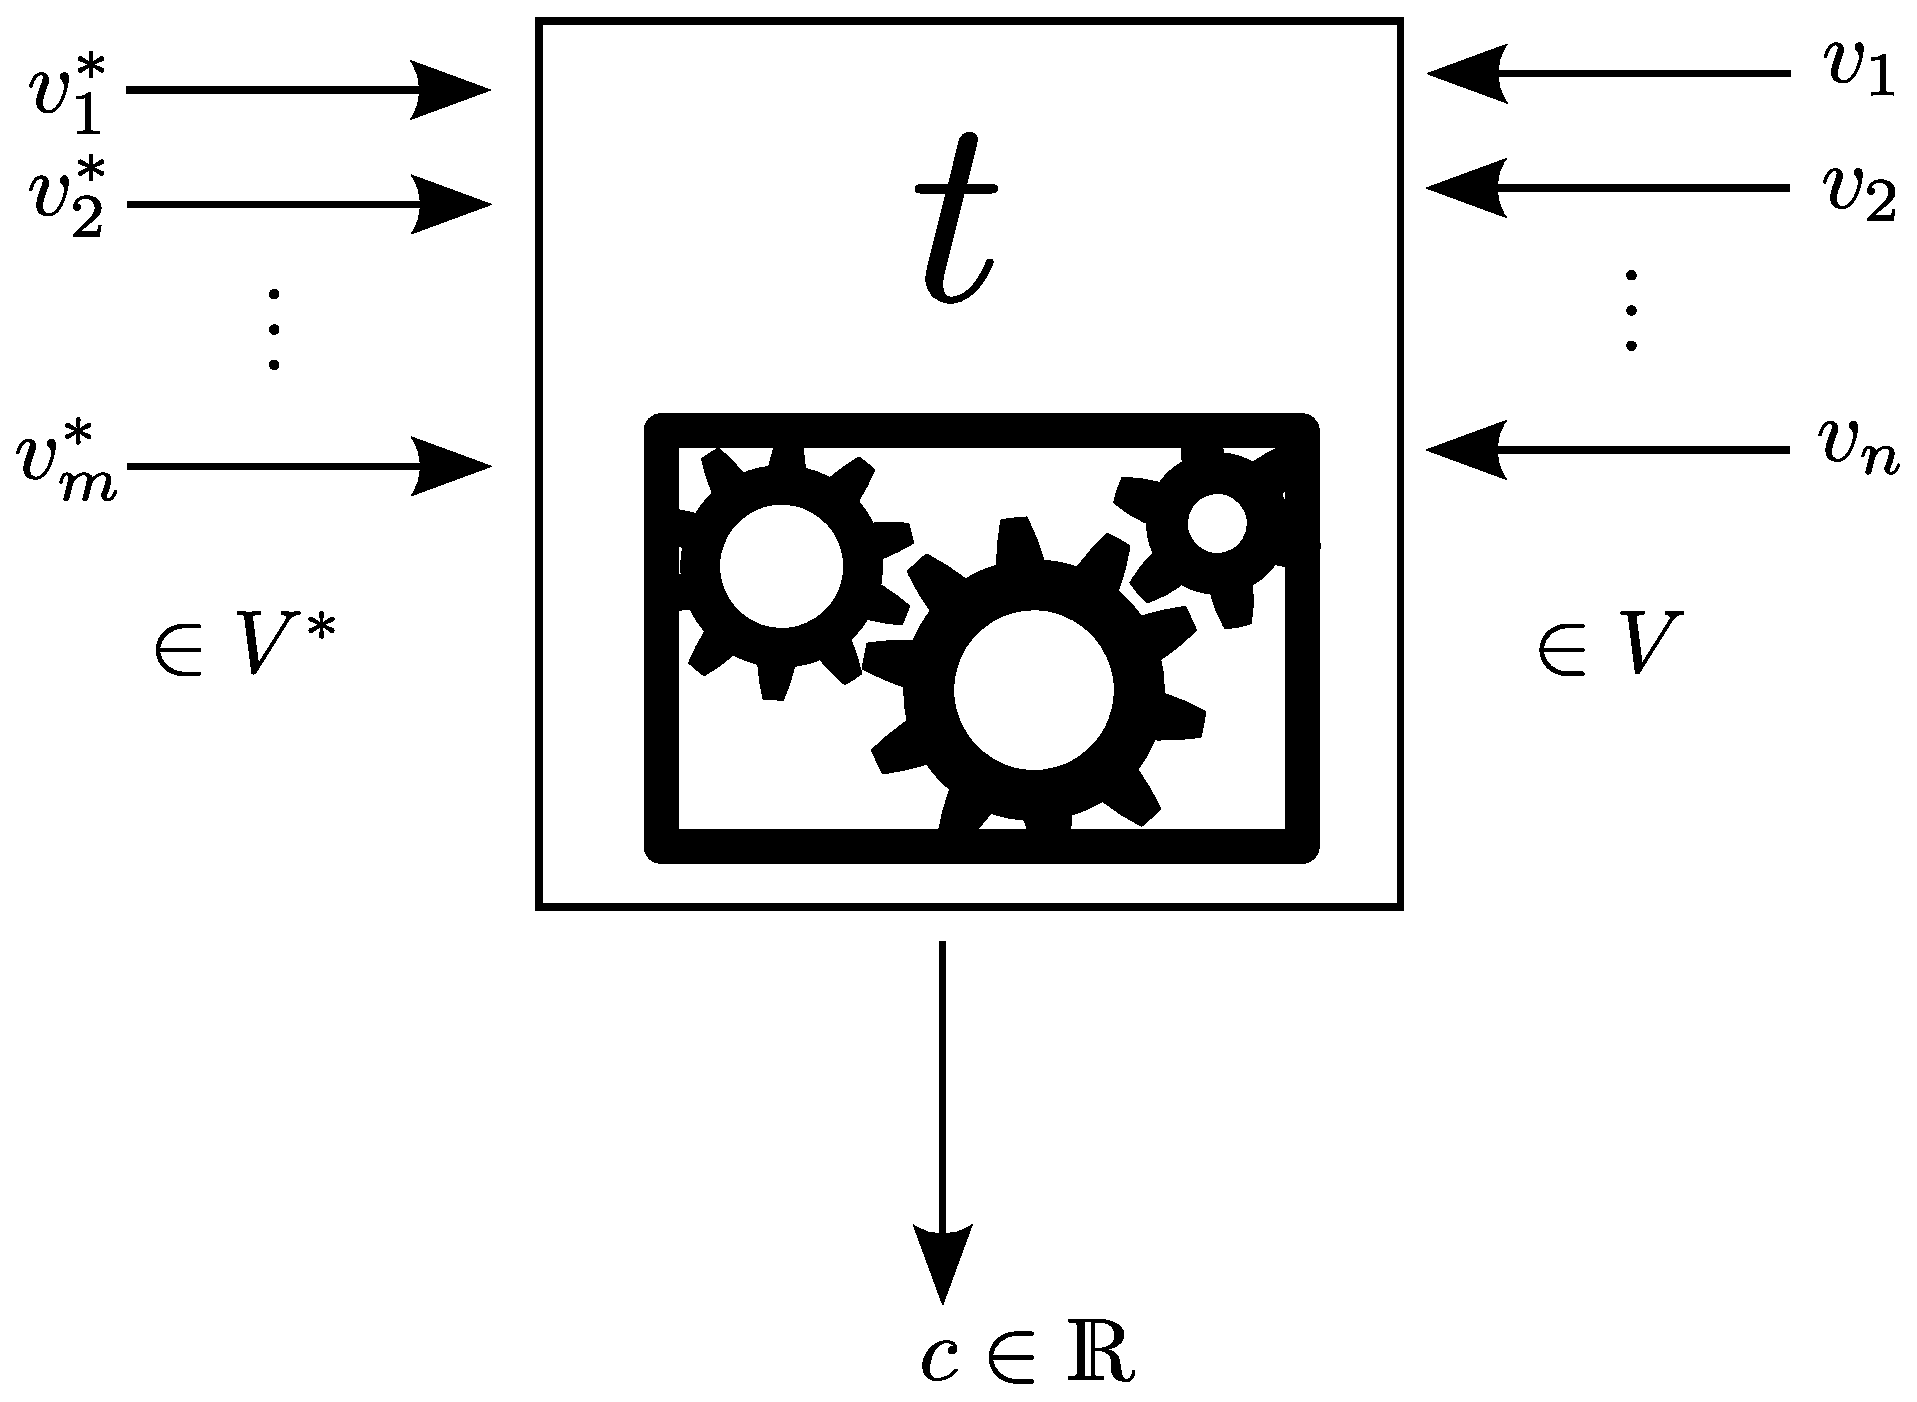
\includegraphics[height=0.7\textheight]{bilder/tensormaschine/Tensor.eps}
    \end{block}
  \end{frame}

  \begin{frame}
    \begin{block}{Differentialform als "`Tensor-Maschine"'}
      Eine Differentialform vom Grad \( n \) ist ein antisymmetrischer \( (0,n) \)-Tensor.

      \centering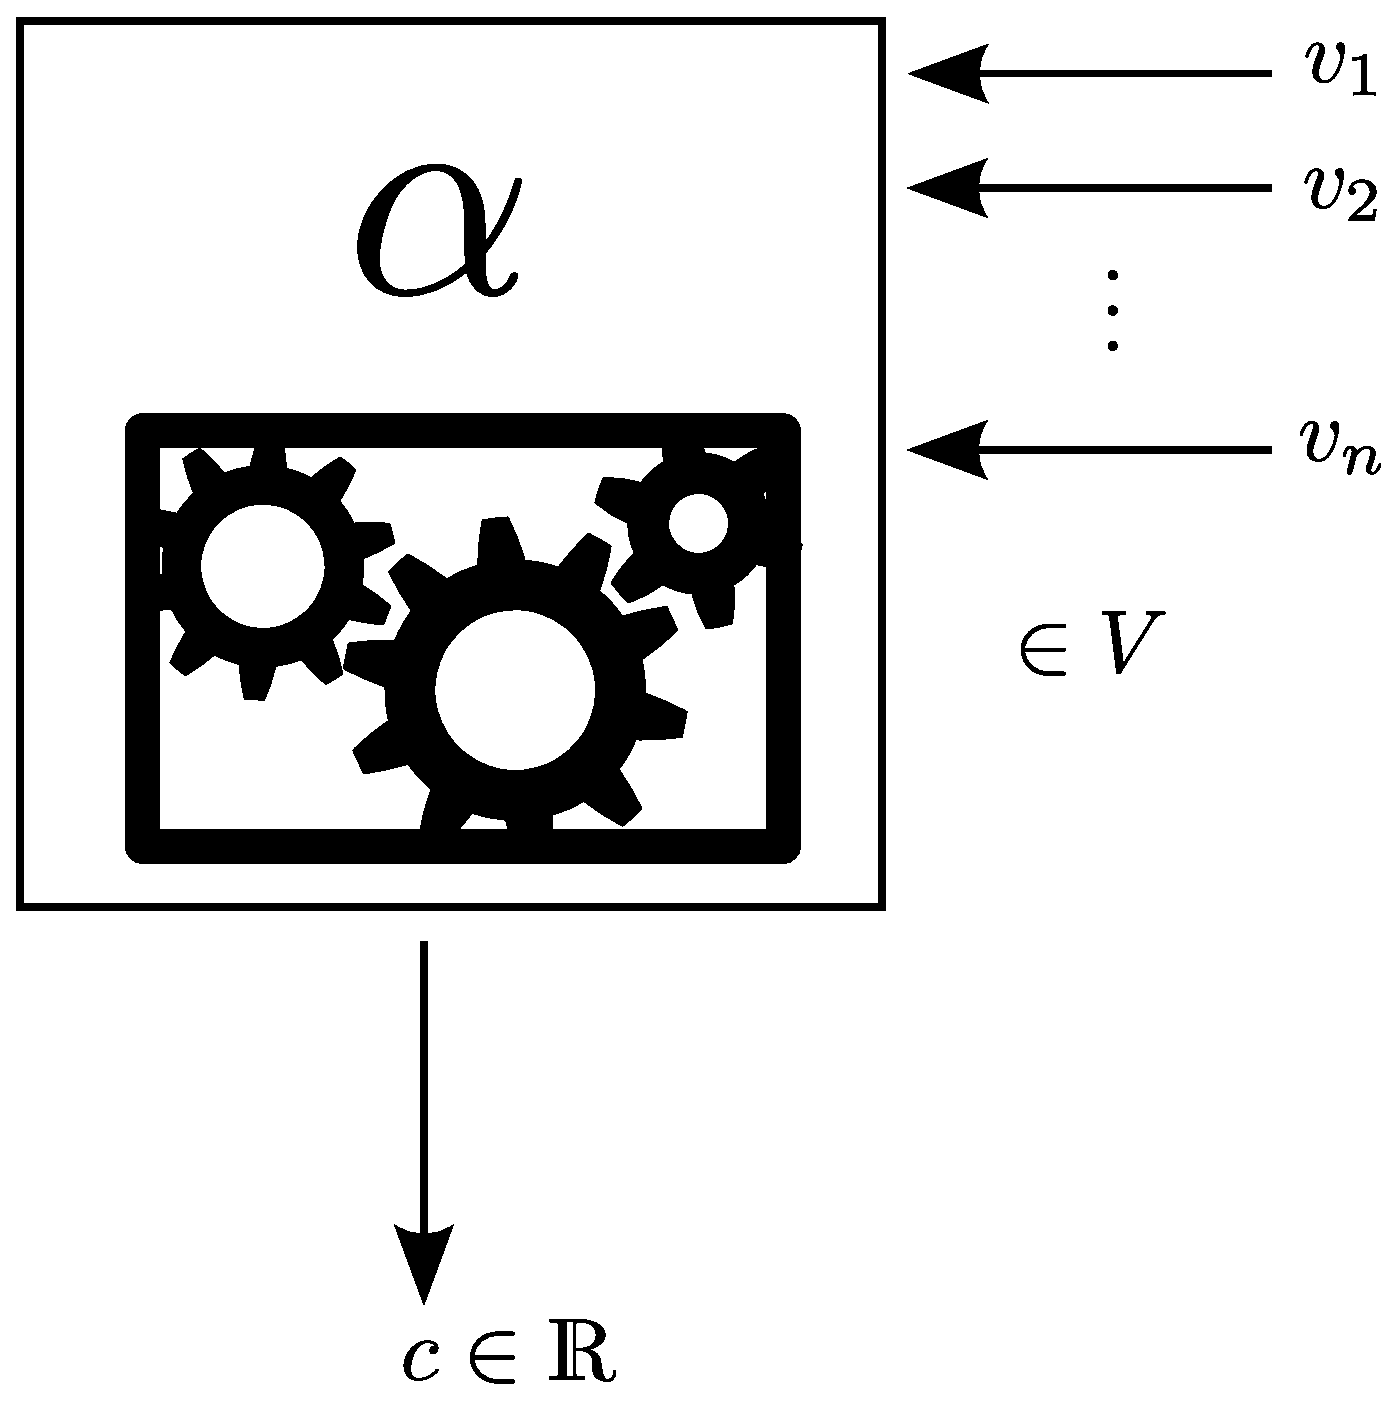
\includegraphics[height=0.7\textheight]{bilder/tensormaschine/Differentialform.eps}
    \end{block}
  \end{frame}

  \begin{frame}
    \begin{block}{Beispiel im \( \R^{2} \supseteq U\)}
      \begin{description}
        \item[0-Formen] \( f:\emptyset\rightarrow\R \) sind Skalare 
          bzw. Funktionen.
          \begin{align*}
            f:U\rightarrow\R,\ x\mapsto f_{x}:=f(x) \formpunkt
          \end{align*}
        \item[1-Formen] \( \alpha\in\left( \R^{2} \right)^{*}\cong\R^{2}  \) können als Zeilenvektoren
          aufgefasst werden
          \begin{align*}
            \alpha = \left[ \alpha_{1},\alpha_{2} \right]:\R^{2}&\rightarrow\R \\ 
                   \vec{v} = \begin{bmatrix}
                    v^{1} \\ v^{2}
                   \end{bmatrix}
                   &\mapsto \alpha(v) = \left[ \alpha_{1},\alpha_{2} \right] \begin{bmatrix}
                          v^{1} \\ v^{2}
                          \end{bmatrix}
                   = \alpha_{1}v^{1} + \alpha_{2}v^{2}
          \end{align*}
          bzw. als Zeilenvektorfeld
          \begin{align*}
            \alpha: U\times\mathcal{V}(U)\rightarrow\R,\ 
                  \left( x,\vec{v} \right)\mapsto\alpha_{x}(\vec{v})=\alpha(x)\vec{v}(x)
          \end{align*}
        \item[2-Formen] können als antisymmetrische Matrizen aufgefasst werden.
      \end{description}
    \end{block}
  \end{frame}

\end{document}
